\section{Rok's Local Volume Mechanism}

Local data on a node need a mechanism to be backed up if the node gets removed
from the cluster; otherwise, the data will be permanently lost, and the user
will not be able to recover them.

Rok provides a mechanism that enables the functionality of moving volumes around
the nodes of a cluster. It leverages an external storage system, such as
Amazon's S3, where it snapshots the local volumes and can restore them on a
different node. Rok refers to moving a local volume to Amazon S3 as
\textit{``Unpinning''} and restoring the volume to a different node as
\textit{``Pinning''}. We describe this mechanism in greater depth in the
following section.

\subsection{Rok Volume Pinning and Unpinning}

\label{section:rok-volume-pinning}

When a local volume is provisioned on a node, the corresponding
\co{PersistentVolume} object on the API Server that represents the volume has
node affinity on it (see section \ref{section:background-pv-node-affinity}). In
the case of local storage, the Rok CSI driver sets the node affinity of the PV
to match only with the node where the local volume is provisioned.


Rok introduces the following terms:
\begin{itemize}
	\tightlist

	\item \textit{Pinned PV}: A PV representing a node's local volume. This PV
	      has node affinity to indicate that it is accessible only from that
	      particular node.
	\item \textit{Unpinned PV}: A PV representing a local volume migrated to S3.
	      The PV has an empty node affinity to indicate that it is accessible
	      from every cluster node.
\end{itemize}

A pinned PV can become unpinned with the process of ``\textit{unpinning}''. An
unpinned PV can become pinned with the process of ``\textit{pinning}''. The
process can be repeated multiple times, essentially allowing the volume to move
around the cluster nodes as many times as needed.

\label{section:design-unpin}
The Rok CSI Controller implements the following mechanism for the unpinning of a
PV:
\begin{enumerate}
	\tightlist
	\item Watches for nodes that are marked unschedulable.
	\item Finds volumes on the unschedulable node that are not currently used by
	      any Pods.
	\item Starts the unpinning process of the unused PV: it takes snapshots of
	      the volume on Amazon S3.
	\item Removes the node affinity from the PV. Note that the \co{nodeAffinity}
	      field of a PV is immutable, i.e., it is not allowed to change. To
	      overcome this restriction, Rok deletes the PV and instantaneously
	      recreates it.
\end{enumerate}

Rok implements the following mechanism for the pinning of a PV:
\begin{enumerate}
	\tightlist
	\item The Scheduler schedules the Pod that references the unpinned PV
	      (through a PVC).
	\item The Kubernetes \co{attachDetach} controller creates a
	      \co{VolumeAttachment} object to signal the external attacher to attach
	      the volume on the node.
	\item The external attacher sees the VolumeAttachment and issues a
	      \co{ControllerPublishVolume} call to the Rok CSI controller.
	\item The Rok CSI controller creates a logical volume on the Rok VG and
	      restores the data of the PV from the Amazon S3 to the logical volume.
	\item The Rok CSI controller sets the appropriate node affinity on the PV to
	      indicate its only accessible from the node the volume was restored to.
\end{enumerate}


\subsection{Rok's Local Volume Protection Mechanism}
\label{section:background-rok-csi-guard}

The Kubernetes maintenance and upgrade tools rely on the \co{drain} operation
(see \ref{section:cordon-drain}). Essentially, before taking any actions to
remove or upgrade a node in the cluster, the tools drain the node (\co{kubectl
	drain}) in order to mark the node unschedulable and safely evict all the Pods.
The Cluster Autoscaler also uses the drain operation before removing a node.

Rok deploys a mechanism to facilitate the upgrades of a cluster and ensure that
the nodes are not removed before Rok snapshots all their local volumes.

The mechanism leverages Pods with properly configured PodDisruptionBudgets to
block their eviction. It relies on the fact that the drain operation fails as
long as the eviction of a Pod fails. The mechanism works as follows:

\begin{enumerate}
	\tightlist
	\item The Rok Operator creates a \co{Deployment} resource \textit{for each
		      node} in the cluster. The Deployment of each node creates
	      \textit{exactly} one replica Pod with node affinity that matches
	      only the specific node. Rok names these Pods  ``\textit{CSI Guard
		      Pod}'', since they protect the node's local volumes.
	\item The Rok Operator creates a \co{PodDisruptionBudget} object for each
	      Rok CSI Guard Deployment. The PodDisruptionBudget demands at any time
	      to exist at least one Rok CSI Guard Pod of the Deployment. This
	      configuration causes any evictions of the Rok CSI Guard Pod to fail.
	\item The drain operation marks the node unschedulable and starts evicting
	      the Pods on the node. The eviction of the CSI Guard fails because of
	      the configured PodDisruptionBudget.
	\item The Rok Operator checks if the Rok CSI has unpinned all the volumes of
	      the unschedulable node; if this condition holds, it removes the
	      PodDisruptionBudget that corresponds to the CSI Guard of the node.
	\item Since the PodDisruptionBudget does not exist anymore, the eviction of
	      the  Rok CSI Guard Pod finally succeeds, and the drain operation
	      completes.
\end{enumerate}

The mechanism is illustrated in Figure ~\ref{figure:rok-csi-guards}.

\clearpage
\vspace*{2cm}
\begin{figure}[H]
	\centering
	\makebox[\textwidth][c]{
		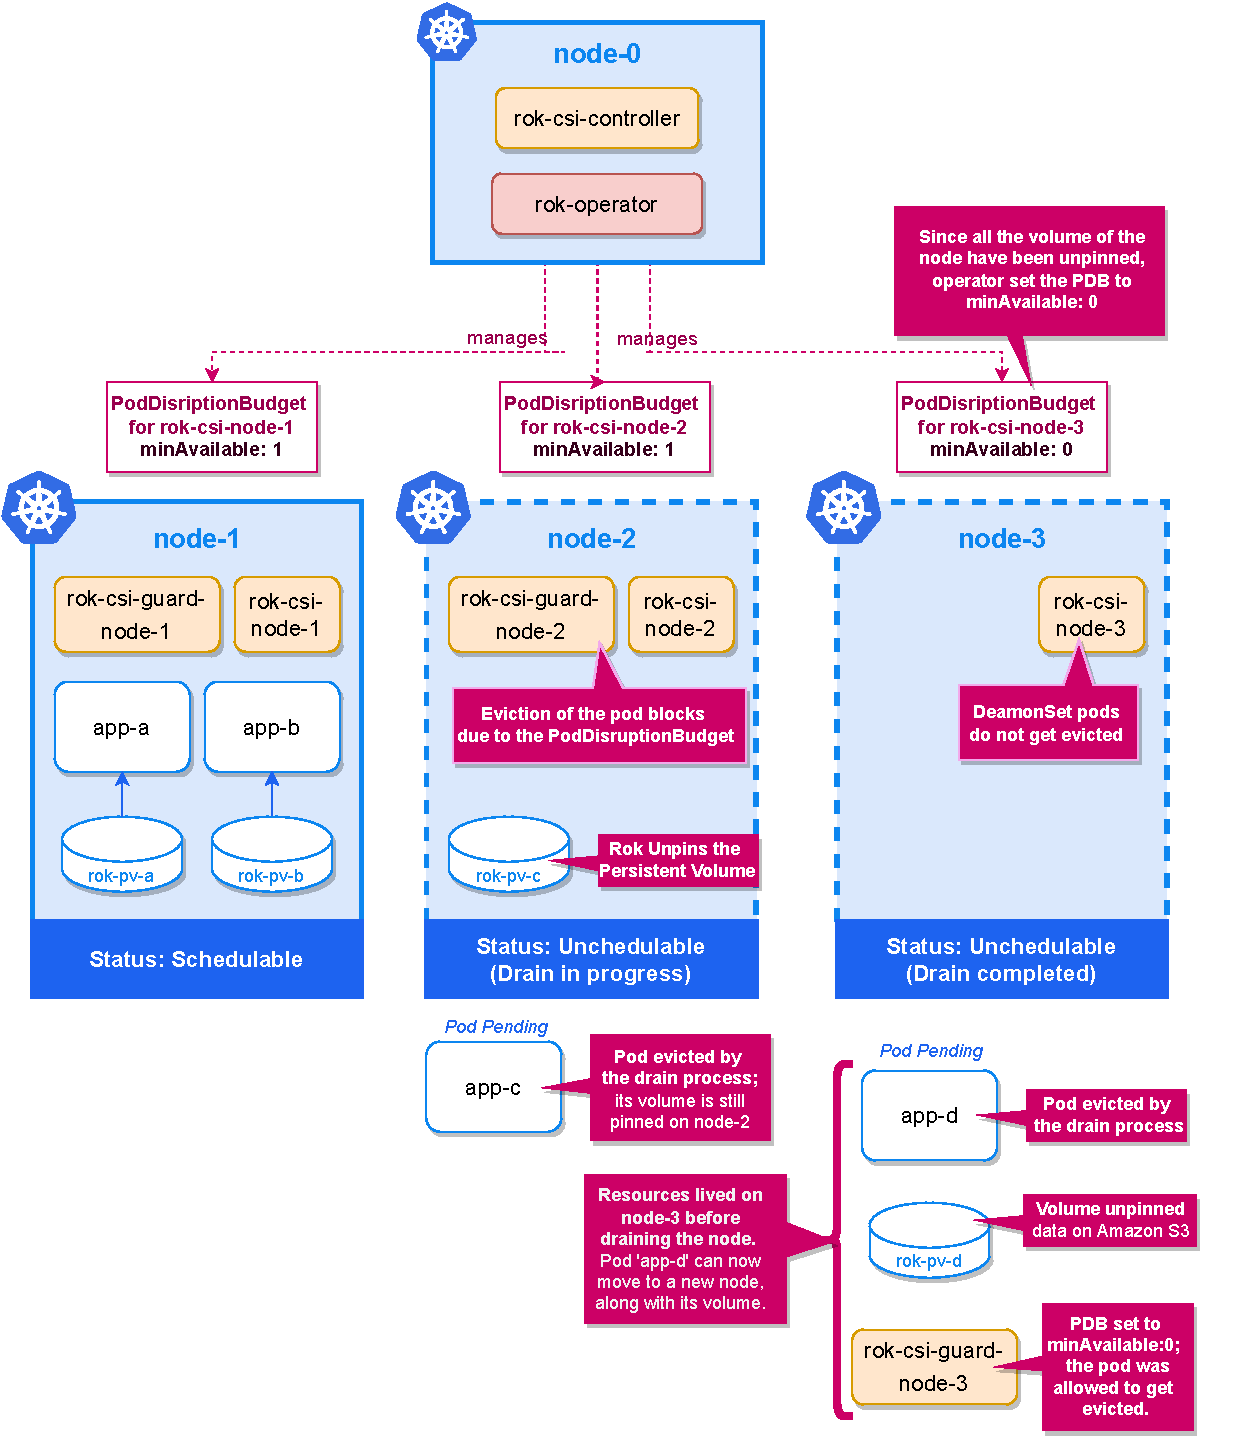
\includegraphics[width=1.2\textwidth]{resources/drain-cluster.pdf}
	}
	\caption{Protecting Local Data with Rok CSI Guard Pods}
	\label{figure:rok-csi-guards}
\end{figure}
\clearpage